% Template for ICIP-2022 paper; to be used with:
%          spconf.sty  - ICASSP/ICIP LaTeX style file, and
%          IEEEbib.bst - IEEE bibliography style file.
% --------------------------------------------------------------------------
\documentclass{article}
\usepackage{spconf,amsmath,graphicx}

% Example definitions.
% --------------------
\def\x{{\mathbf x}}
\def\L{{\cal L}}

% Title.
% ------
\title{AUTOMATICALLY RESIZING VIDEO TO FOCUS ON SPEAKERS}
%
% Single address.
% ---------------
\name{Benjamin Smidt, Johann Ramirez}
\address{Clips AI}
%
% For example:
% ------------
%\address{School\\
%	Department\\
%	Address}
%
% Two addresses (uncomment and modify for two-address case).
% ----------------------------------------------------------
%\twoauthors
%  {A. Author-one, B. Author-two\sthanks{Thanks to XYZ agency for funding.}}
%	{School A-B\\
%	Department A-B\\
%	Address A-B}
%  {C. Author-three, D. Author-four\sthanks{The fourth author performed the work
%	while at ...}}
%	{School C-D\\
%	Department C-D\\
%	Address C-D}
%
\begin{document}
%\ninept
%
\maketitle
%
\begin{abstract}
This paper introduces a novel algorithm for automatically resizing videos to focus on the current speaker. With the rise of mobile devices and social media, there's an increasing demand for transforming horizontally formatted videos into vertically formatted ones, particularly for audio-centric videos such as podcasts or interviews. This approach leverages the latest techniques in speaker diarization, face detection, and facial landmark detection. Although quite effective, the algorithm has noticeable limitations in cases of small faces, excessive non-speaker mouth movement, and occluded faces. Future work needs to be done on dataset curation for algorithm evaluation, addressing identified failure cases, and enhancing memory and speed efficiency.
\end{abstract}
\section{INTRODUCTION}
\label{sec:intro}

Owing to the success of mobile devices and social media, short-form videos (less than one minute) have emerged as a dominant modality for media consumption. This surge in popularity presents a need for converting media into a short-form ready format. One vital requirement is a vertical aspect ratio. As such, large amounts of video with a horizontal aspect ratio are being resized to a vertical aspect ratio. The difficult step in this conversion is selecting what to focus on. Audio-centric videos (such as podcasts) are a large subset of the videos needing to be resized. Given these videos typically record the speakers, such videos can simply be resized to focus on whoever is speaking.

\begin{figure}[htb]
    \begin{minipage}[b]{1.0\linewidth}
        \centering
        \centerline{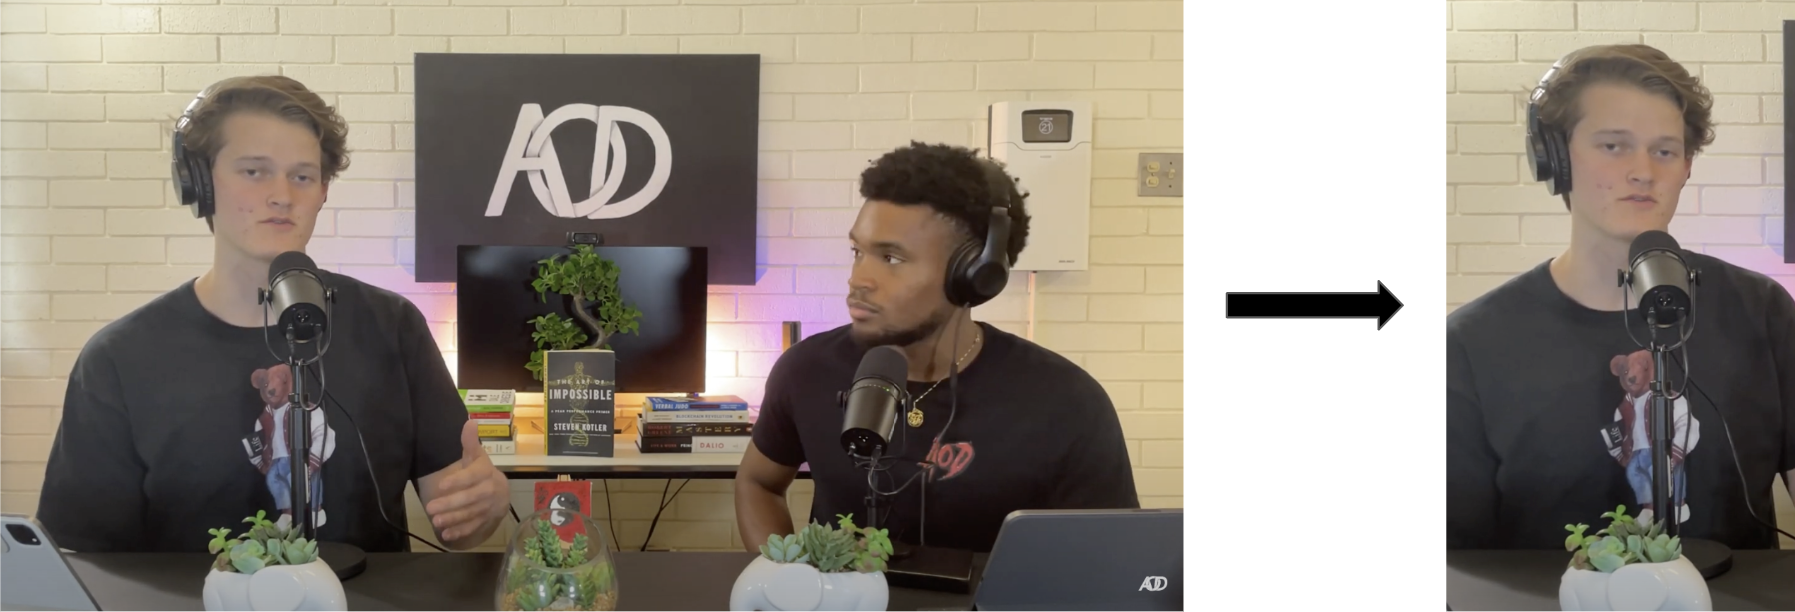
\includegraphics[width=8cm]{horizontal-to-vertical-example.png}}
        \medskip
    \end{minipage}
    \caption{Example of resizing a video to focus on the current speaker}
    \label{fig:horizontal-to-vertical-example}
    \end{figure}

This paper introduces a novel algorithm automating the resizing of videos to focus on the video's current speaker. Traditionally, this resizing process has been a manual and time-consuming task. But the advent of deep learning and advanced image processing techniques lay the groundwork for a promising solution.

Initially this algorithm was created with the intent of resizing horizontal podcast videos (16:9 aspect ratio) to vertical videos (9:16 aspect ratio). However, arbitrary input and output aspect ratios may be leveraged. Furthermore, the applicability of this algorithm extends well beyond podcasts to various forms of other audio-centric videos including interviews, speeches, sermons, and the like.

\section{METHODS}
\label{sec:pagestyle}

\subsection{Definitions}
We begin by defining some notation. Let $V$ be a set of all frames in a video. Let $f_i \in V$ be frame $i$ in video $V$ where $1 \le i \le |V|$. Note that frame $f_{i-1}$ is the frame just before $f_i$ and $f_{i+1}$ the frame just after $f_i$. The indices of the frames in $V$ are ordered chronologically. Let a segment $S \in V$ be a subset of frames in $V$ forming a continuous time slice (with no gaps) of the video. That is, if the first frame in $S$ is $f_a$ and the last frame is $f_b$, then $f_i$ belongs to $S$ if and only if $a \le i \le b$.

\subsection{Determining Segments}
\label{ssec:determining-segments}
Our first step is to determine segments $S_1, ..., S_t$ that form a partition of $V$ where $1 \le t \le |V|$ such that all frames in a given segment can be resized to the exact same location in the video. Note that, while $t$ could be equal to $|V|$ (each frame requires a resizing location), in practice $t << |V|$ which is crucial for minimizing the amount of downstream processing. We'll find these segments by obtaining data about: 1) distinct speaker segments in which a single speaker is talking uninterrupted 2) distinct scene segments in which no drastic scene cuts occur.

The first indicator of distinct segments is the speaker diarization data of the video's audio. We assume that a new individual speaking indicates a need to reposition the focus of the resized video. Speaker diarization data can be obtained by the \emph{pyannote/speaker-diarization-3.0} model offered by pyannote.audio \cite{Plaquet23} \cite{Bredin23}. Feeding the video's extracted audio into pyannote.audio returns segments of the video, labelled with who is speaking throughout that segment. We'll call the segments derived from pyannote.audio \emph{speaker segments}. 

Of course, speakers occasionally talk at the same time or pauses occur in which no speaker is talking. Thus, the speaker segments do not form a partition of $V$. Some segments overlap and some frames of the video do not belong to any segment. To correct this, simple heuristic choices can be implemented to massage the segments returned by pyannote.audio into a partition of segments $S_1, ..., S_p$ where $1 \le p \le |V|$ and $p$ denotes the number of speaker segments in the video. Again $p << |V|$.

\begin{figure}[htb]
\begin{minipage}[b]{1.0\linewidth}
    \centering
    \centerline{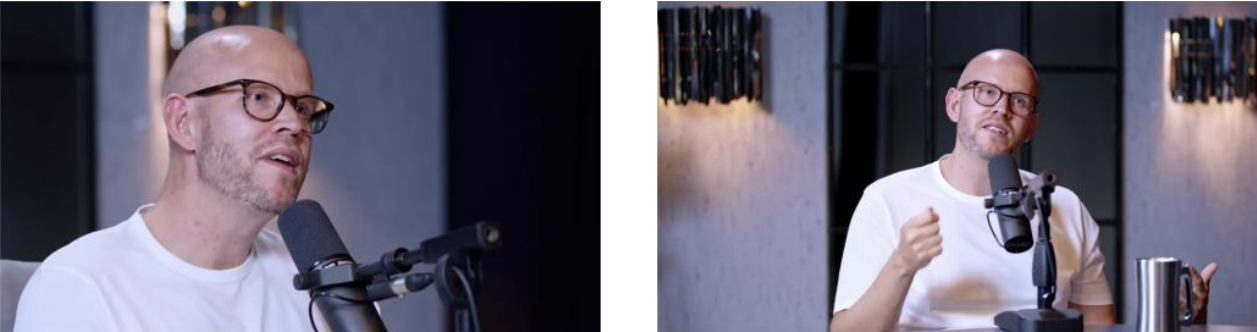
\includegraphics[width=8.5cm]{scene-segment.png}}
    \centerline{Camera 1 \; \; \; \; \; \; \; \; \; \; \; \; \; \; \; \; Camera 2}
    \medskip
\end{minipage}
\caption{Example of a scene change while a single speaker is talking.}
\label{fig:scene-segment}
\end{figure}

However, the speaker segments are not the only indicators of a need to reposition the focus of the resized video. \textbf{Figure \ref{fig:scene-segment}} shows two frames from the same video only a few milliseconds apart. Although the same speaker is talking, the video cuts from camera 1 to camera 2. Since the speaker is no longer located in the same position, the scene cut indicates a need to reposition the focus of the resized video.

These drastic scene cuts can be detected using PySceneDetect \cite{PySceneDetect}. Feeding the video into PySceneDetect returns timestamps of all the scene cuts in the video. These scene cuts are considered boundaries between \emph{scene segments} $S_1, ..., S_c$ where $c$ denotes the number of scene segments in the video. Again $c << |V|$.

With our speaker segments and scene segments in hand, we merge them together to form segments $S_1, ..., S_t$ where $p, c \le t \le |V|$. The rest of the alogrithm assumes each segment contains a set of frames which can all be resized to the same location in the video. In practice this assumption holds very well for media such as podcasts, interviews, and the like. 


\subsection{Locating and Grouping Faces}
\label{ssec:locating-and-grouping-faces}

After determining the speaker segments $S_1, ..., S_t$, we need to locate the speaker within each segment. This is done in two steps: 1) identify the faces in a segment 2) determine which face is speaking.

Before identifying the faces in each segment, we first sample $n$ frames from each segment. Instead of analyzing all frames in a segment, we only analyze these samples to minimize the amount of processing. Since there are $t$ segments and $n$ samples per segment, at most $tn$ frames are analyzed throughout the rest of the algorithm. $tn$ is an upperbound since some segments may not have $n$ frames (they may be particularly short). In practice $n = 13$ works quite well.

Next we'll use the $n$ sample frames from each segment to determine all the faces in each segment. Many face detection models exist. I chose to use facenet-pytorch \cite{FacenetPyTorch} \cite{Facenet} \cite{VGGFace2} \cite{FaceRepresentation} \cite{CascadedConvolution}, an implementation adapted from facenet (an implementation written with TensorFlow) \cite{FacenetTensorFlow}. Each sample frame is fed into facenet-pytorch which returns two coordinates-- the upper left corner and the bottom right corner of every face's bounding box. If the upper left corner is denoted by $(x_1, y_1)$ and the bottom right corner by $(x_2, y_2)$, facenet-pytorch would return a tuple of $(x_1, y_1, x_2, y_2)$.

\begin{figure}[htb]
\begin{minipage}[b]{1.0\linewidth}
    \centering
    \centerline{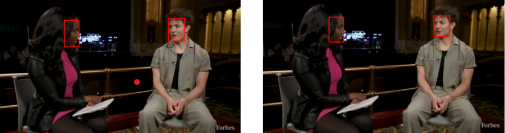
\includegraphics[width=8.5cm]{sample-face-detections.png}}
    \medskip
\end{minipage}
\caption{Two sample face detections from a video segment.}
\label{fig:sample-face-detections}
\end{figure}

Identifying the faces in each frame is key. However, to determine who is speaking in a given segment, we'll need to group the faces throughout the $n$ sample frames. For instance, if there are three faces in each of the $n$ sample frames, we'd desire three groups: face 1 across all $n$ frames, face 2 across all $n$ frames, and face 3 across all $n$ frames.

\begin{figure}[htb]
\begin{minipage}[b]{1.0\linewidth}
    \centering
    \centerline{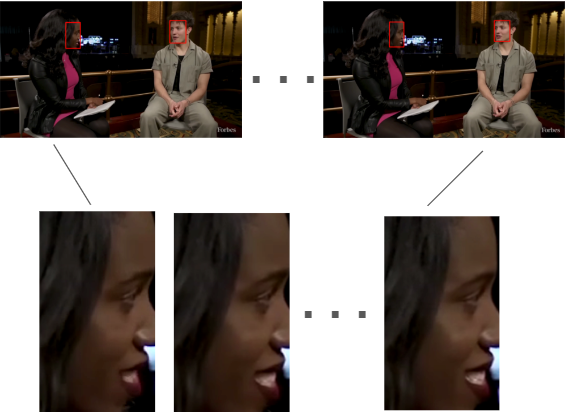
\includegraphics[width=8.5cm]{k-means-face-detections.png}}
    \medskip
\end{minipage}
\caption{Grouping of face 1 across $n$ sample frames of a video segment using k-means.}
\label{fig:k-means-face-detections}
\end{figure}

This can be done very effectively using k-means. Since faces rarely move much throughout a segment (if at all), clustering the faces according to the bounding box coordinates given by the facenet-pytorch yields quick and reliable results. For a given segment, $k$ should be set to the maximum number of faces detected in any sample frame in that segment.

\subsection{Determining the Speaker}
The final step is to determine which of the faces in the segment is the one speaking. To do so I used MediaPipe's face landmarks detection to locate the position of the lips on every face \cite{MediaPipe}.
\begin{figure}[htb]
\begin{minipage}[b]{1.0\linewidth}
    \centering
    \centerline{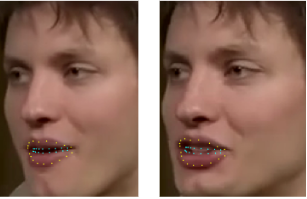
\includegraphics[width=8.5cm]{face-landmarks.png}}
    \medskip
\end{minipage}
\caption{Example mouth landmarks detected using MediaPipe.}
\label{fig:face-landmarks}
\end{figure}

From the mouth landmarks given by MediaPipe, we can calculate the Mouth Aspect Ratio (MAR). This is a measure of the width:height ratio of the mouth. Using the labelled points in \textbf{Figure \ref{fig:MAR}}, the equation is as follows \cite{MAR}.

\[ MAR = \frac{\sum_{i=1}^9 \|p_{i} - p_{i+9}\|}{9\|p_{20} - p_{19}\|} \]

\begin{figure}[htb]
\begin{minipage}[b]{1.0\linewidth}
    \centering
    \centerline{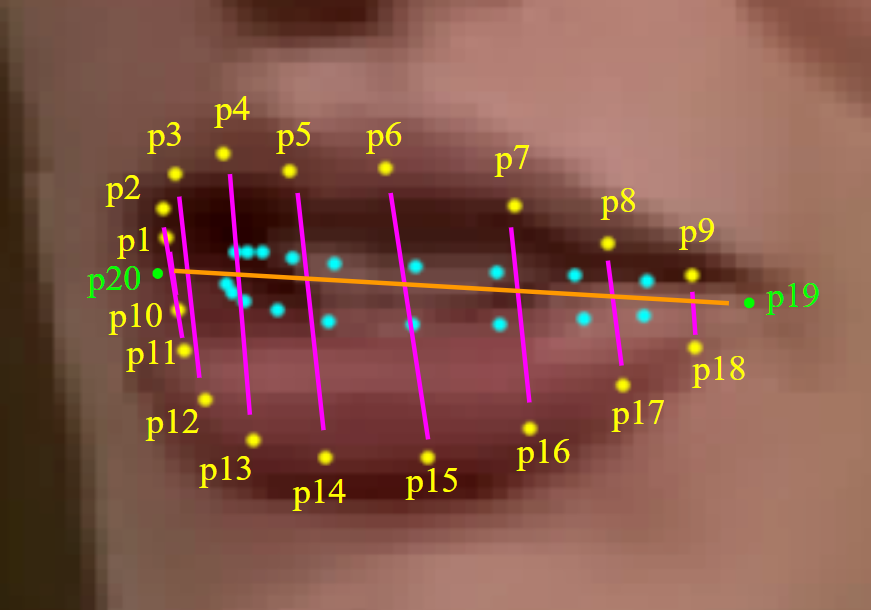
\includegraphics[width=8.5cm]{MAR.png}}
    \medskip
\end{minipage}
\caption{MediaPipe mouth landmarks for calculating MAR}
\label{fig:MAR}
\end{figure}

For each group of faces in a segment (recall there are $n$ faces in each group, one for each sample), we use the MAR of each face to calculate the Mouth Movement Score (MMS). This has no history in the literature and was created specifically with this algorithm in mind. 

Consider a segment with MAR scores $m_1, ..., m_n$ such that the scores are ordered chronologically. That is, $i < j$ suggests that the $m_i$ belongs to a frame occurring before $m_j$ for any two indices $1 \le i, j \le n$. Then 
\[ MMS = \sum_{i=2}^n{|m_i - m_{i-1}}| \]
The face with the largest MMS scores for a given segment is considered the speaker for that segment. The idea is that a speaker's mouth will constantly move up and down overtime while non-speaker mouths will not. Ordering the MAR scores increases robustness against detecting erroneous mouth movement such as smiling, laughing, or yawning.

Having selected the speaker for every segment, each segment is resized to focus on the center of the segment speaker's face. Concatenating each segment's resized video yields the entire resized video, focusing on the current speaker. Any aspect ratios may be leveraged with this algorithm. However, only a conversion from 16:9 to 9:16 has been tested.

\section{RESULTS}
\label{sec:majhead}

\subsection{Podcasts and Other Applications}
\label{ssec:podcasts-and-other-applications}

Due to constraints on time and resources, no qualitative data can be given about the accuracy of this method. I was unable to ascertain a labelled dataset for this problem and did not have the resources to curate (even a small one) alone. Future work should focus on curating this dataset so that this algorithm, and others, can be improved in a qualitative manner.

Despite these limitations though, it is my opinion that the algorithm is quite robust. Of various tested podcasts, it was rare to see a segment incorrectly positioned. In fact, much more difficult test cases such as standup comedy or the news performed reasonably well given the limitations of the algorithm.

Furthermore, these results are impressive given a machine learning model did not need to be trained. Existing technologies could be leverage algorithmically to achieve the results, yielding a robust system that circumvents the manual collection and training of data. This, of course, is a huge positive since the algorithm can be used as a tool for efficient curation of a dataset for future work.

\subsection{Failure Cases}
\label{ssec:failure-cases}

While the algorithm is successful the overwhelming majority of the time, there were some notable failure cases. The first is for faces that are small relative to the size of the image. This is sometimes the case for speeches or other events where the camera is distanced quite far from the stage. Face detection models, being trained on images of a particular pixel width and height, often have trouble detecting faces who's pixel width and height are far outside their training data.


\begin{figure}[htb]
\begin{minipage}[b]{1.0\linewidth}
    \centering
    \centerline{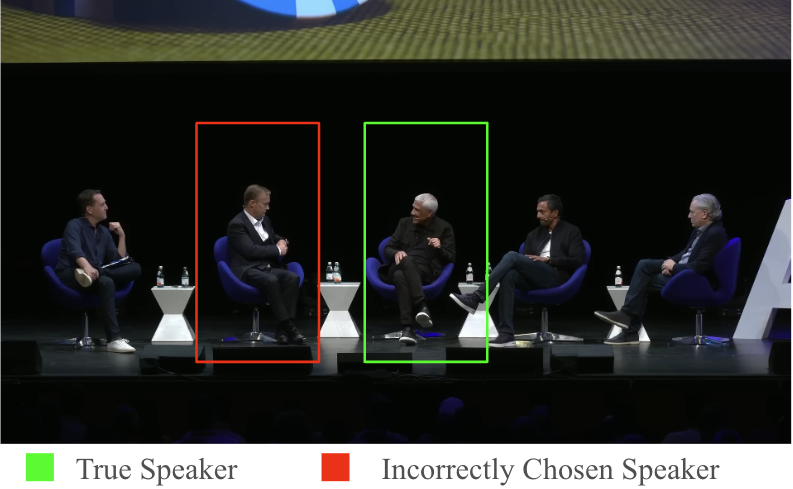
\includegraphics[width=8.5cm]{small-faces.png}}
    \medskip
\end{minipage}
\caption{Incorrectly chosen speaker due to small faces}
\label{fig:small-faces}
\end{figure}

An example of this can be seen in \textbf{Figure \ref{fig:small-faces}}. The face detection model fails to detect the speaker's face at all. As a result, the man to his left is chosen as a substitute in the absence of the true speaker's face being identified in that segment.

\begin{figure}[htb]
\begin{minipage}[b]{1.0\linewidth}
    \centering
    \centerline{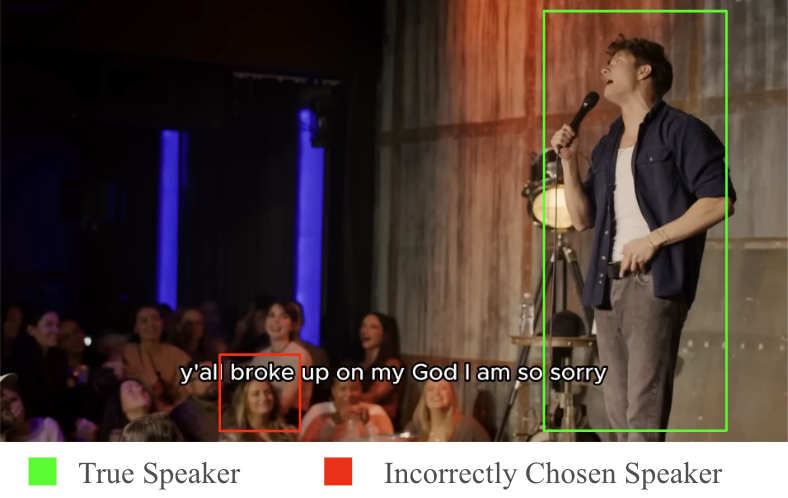
\includegraphics[width=8.5cm]{smiling-face.png}}
    \medskip
\end{minipage}
\caption{Incorrectly chosen speaker due to a non-speaker smiling}
\label{fig:smiling-face}
\end{figure}

Another failure case is when non-speakers are moving their mouth quite a bit. This is generally some form of smiling or laughing and occasionally yawning. As result, the MMS of this non-speaker is quite high, fooling the alogrithm into thinking this non-speaker is the one speaking. An example of this can be seen in \textbf{Figure \ref{fig:smiling-face}}, where the woman is smiling. It's difficult to see in a single frame but her laugh fools the algorithm into selecting her as the speaker instead of the man on stage.

\begin{figure}[htb]
\begin{minipage}[b]{1.0\linewidth}
    \centering
    \centerline{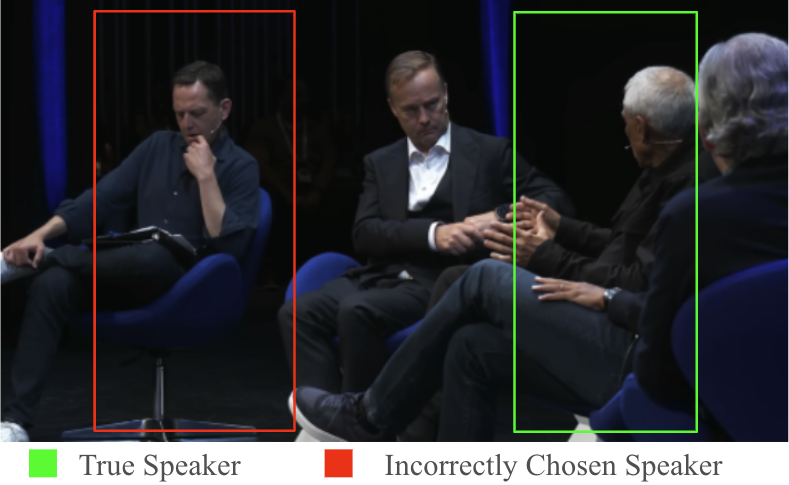
\includegraphics[width=8.5cm]{occluded-face.png}}
    \medskip
\end{minipage}
\caption{Incorrectly chosen speaker due to the speaker's face being occluded}
\label{fig:occluded-face}
\end{figure}

A third failure case is when the speaker's face is heavily occluded. Despite face detection models being quite robust to occlusion, this was still a non-trivial point of failure. Although, as seen in \textbf{Figure \ref{fig:occluded-face}}, this point of failure cannot always be solved by the face detection algorithm. Sometimes the speaker's face is hardly in the picture, if at all. A separate and/or corrective model may be needed to determine the head or body of the speaker in rare cases where the speaker's face is not in the frame.


\subsection{Challenges}
\label{ssec:challenges}
Despite determining homogeneous segments and sampling frames from these segments to minimize processing, memory and speed were still challenges.

\textbf{Figure \ref{fig:memory}} shows the memory requirements just for \emph{extracting the sample frames} from the video used in the algorithm. While this varies widely with the video, one 24 minute video required nearly 8.5 GiB of memory for the extracted sample frames. Yet, large amounts of memory still must be allocated for the different models used in the algorithm, the face detection model requiring particularly large amounts. Obviously batches must be used for videos requiring large amounts of memory. 

\begin{figure}[htb]
\begin{minipage}[b]{1.0\linewidth}
    \centering
    \centerline{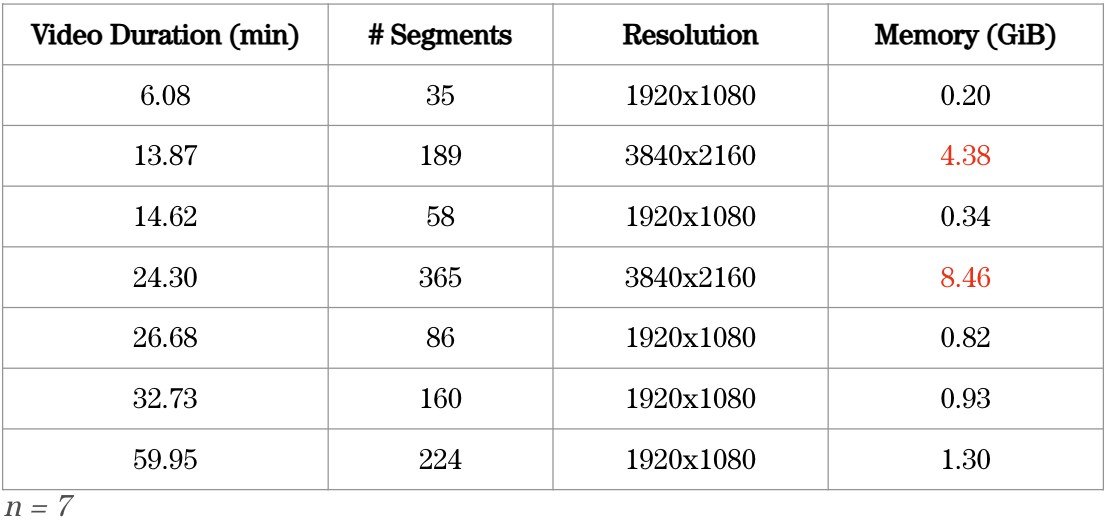
\includegraphics[width=8.5cm]{memory.png}}
    \medskip
\end{minipage}
\caption{Memory requirements for extracting the video sample frames used in the algorithm}
\label{fig:memory}
\end{figure}

\textbf{Figure \ref{fig:speed}} shows the runtime of the algorithm \emph{not including speaker diarization}. Since data for speaker diarization runtimes can easily be found and vary depending the chosen model, I chose not to include it in these results. These numbers are tested with $n = 7$ samples per segment on a Mac Studio with 12 CPU cores using the M2 MAX chip. GPU's were not utilized in these numbers due to incompatibilities with Apple Silicon.

\begin{figure}[htb]
\begin{minipage}[b]{1.0\linewidth}
    \centering
    \centerline{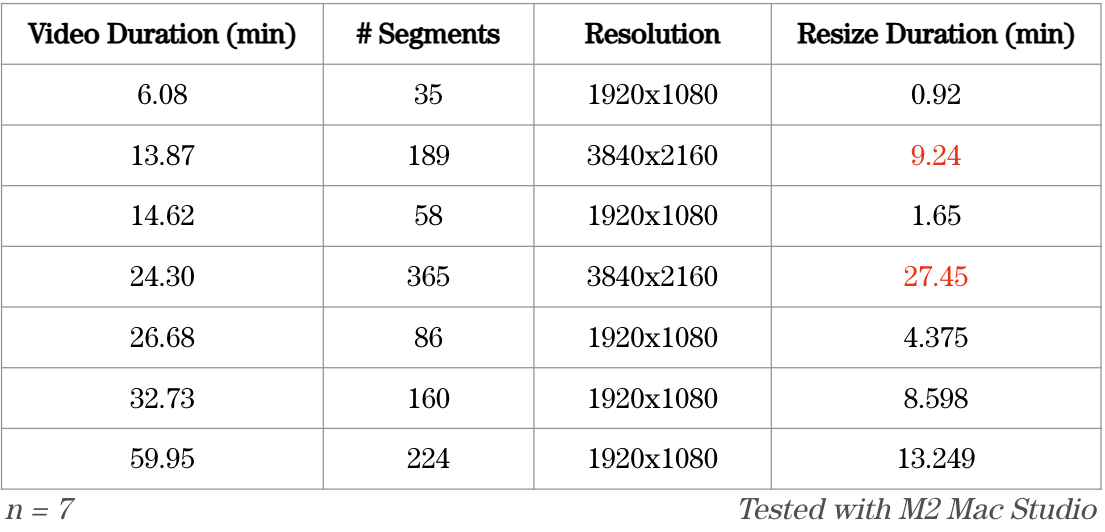
\includegraphics[width=8.5cm]{speed.png}}
    \medskip
\end{minipage}
\caption{Runtime of resizing videos, not including processing of speaker diarization}
\label{fig:speed}
\end{figure}

\section{CONCLUSION}
\label{sec:foot}
In the absence of qualitative data about the accuracy of this algorithm, a conclusion of it's validity cannot be made. However, from watching many resized videos, it's my opinion that the algorithm is quite robust for resizing podcast videos and could be readily applied to adjacent applications such as speeches, interviews, and sermons as well.

Future work should focus on three major points: 1) curating a dataset for evaluating the quality of this algorithm and others 2) correcting the failure cases of the algorithm 3) improving the efficiency of the algorithm regarding memory and runtime. Given my inexperience in machine learning and video processing, I believe significant improvements can be made quickly on all three of these fronts.

% References should be produced using the bibtex program from suitable
% BiBTeX files (here: strings, refs, manuals). The IEEE.bst bibliography
% style file from IEEE produces unsorted bibliography list.
% -------------------------------------------------------------------------
\bibliographystyle{IEEE}
\bibliography{strings,refs}

\end{document}